\chapter{Example Generator Implementations}
To illustrate a few possibilities of BAG generators, we show various circuits of increasing complexity. 
\section{Starting Small: Passive Loaded Differential Amplifier}
A very commonly used block in many ICs is the differential amplifier. In this case the load is passive. The topology is the same as that used in Chapter 4, and can be seen in Figure 4.7. An example generated layout instance is shown in Figure \ref{fig:passive_amp}.
\begin{figure}[h]
\centering
\begin{subfigure}{.8\linewidth}
  \centering
  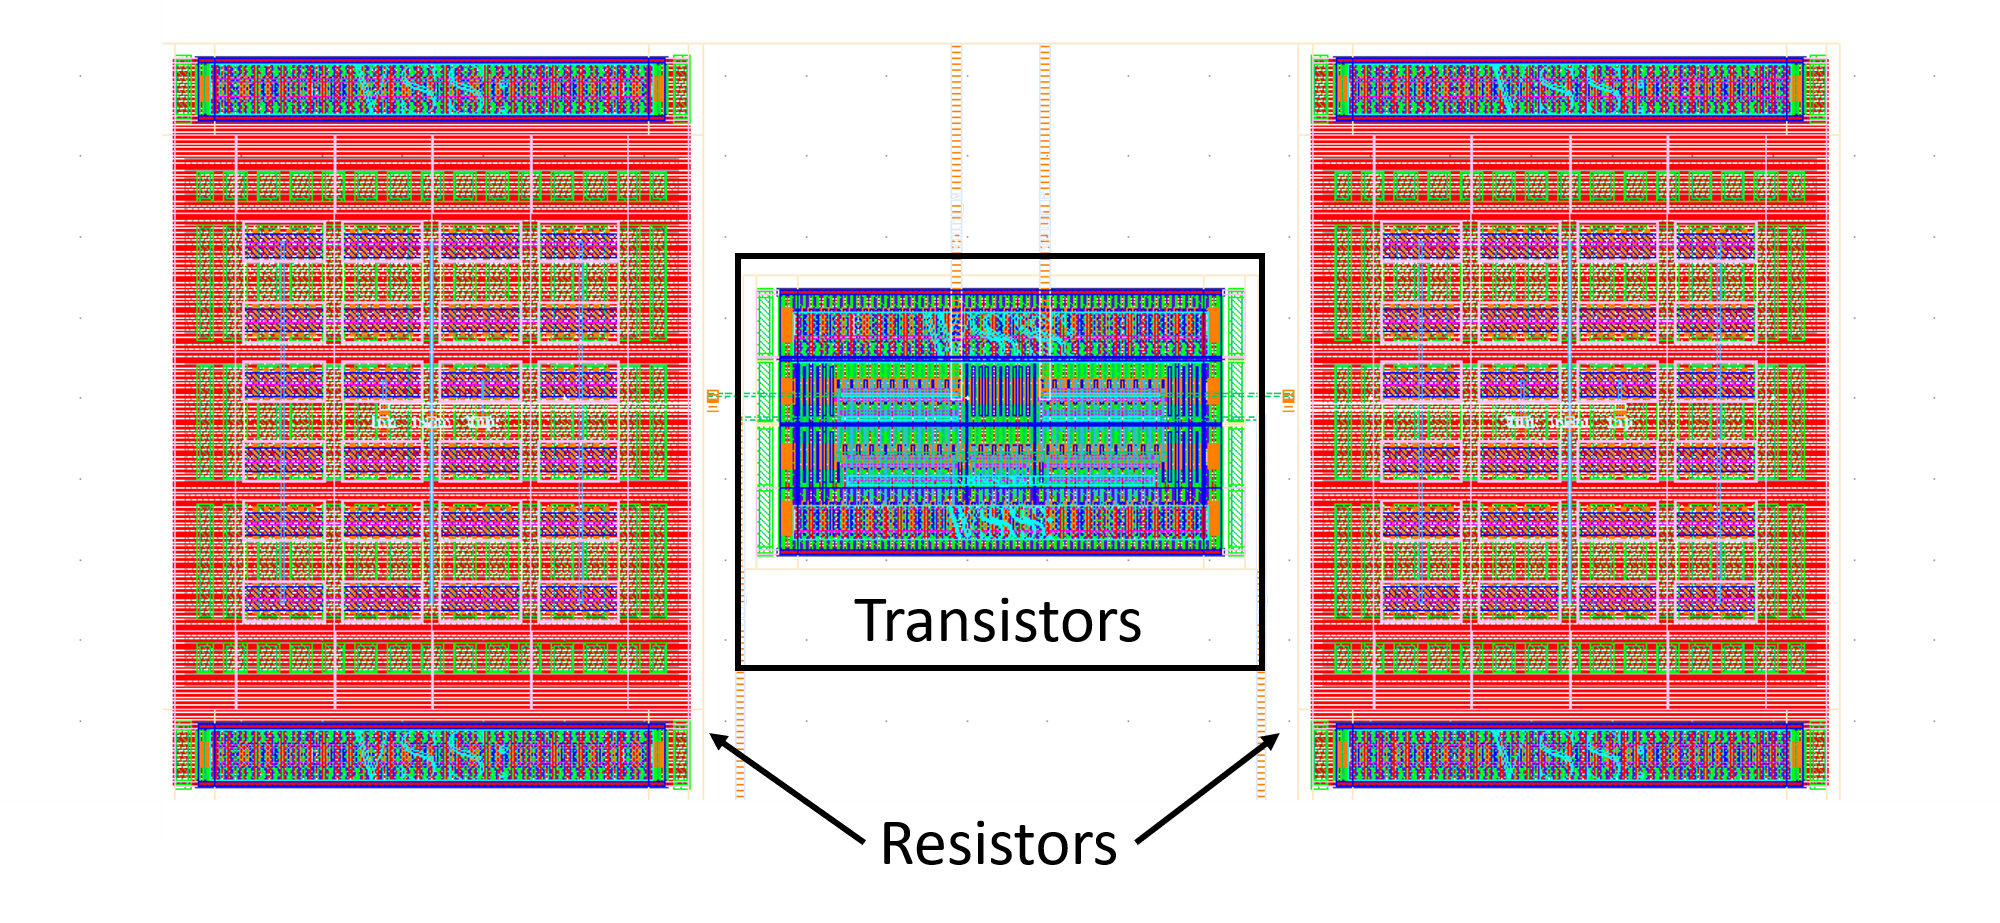
\includegraphics[width=\textwidth]{passive_layout_annotated}
  \caption{Full layout}
  \label{fig:sfig1}
\end{subfigure}
\begin{subfigure}{.8\linewidth}
  \centering
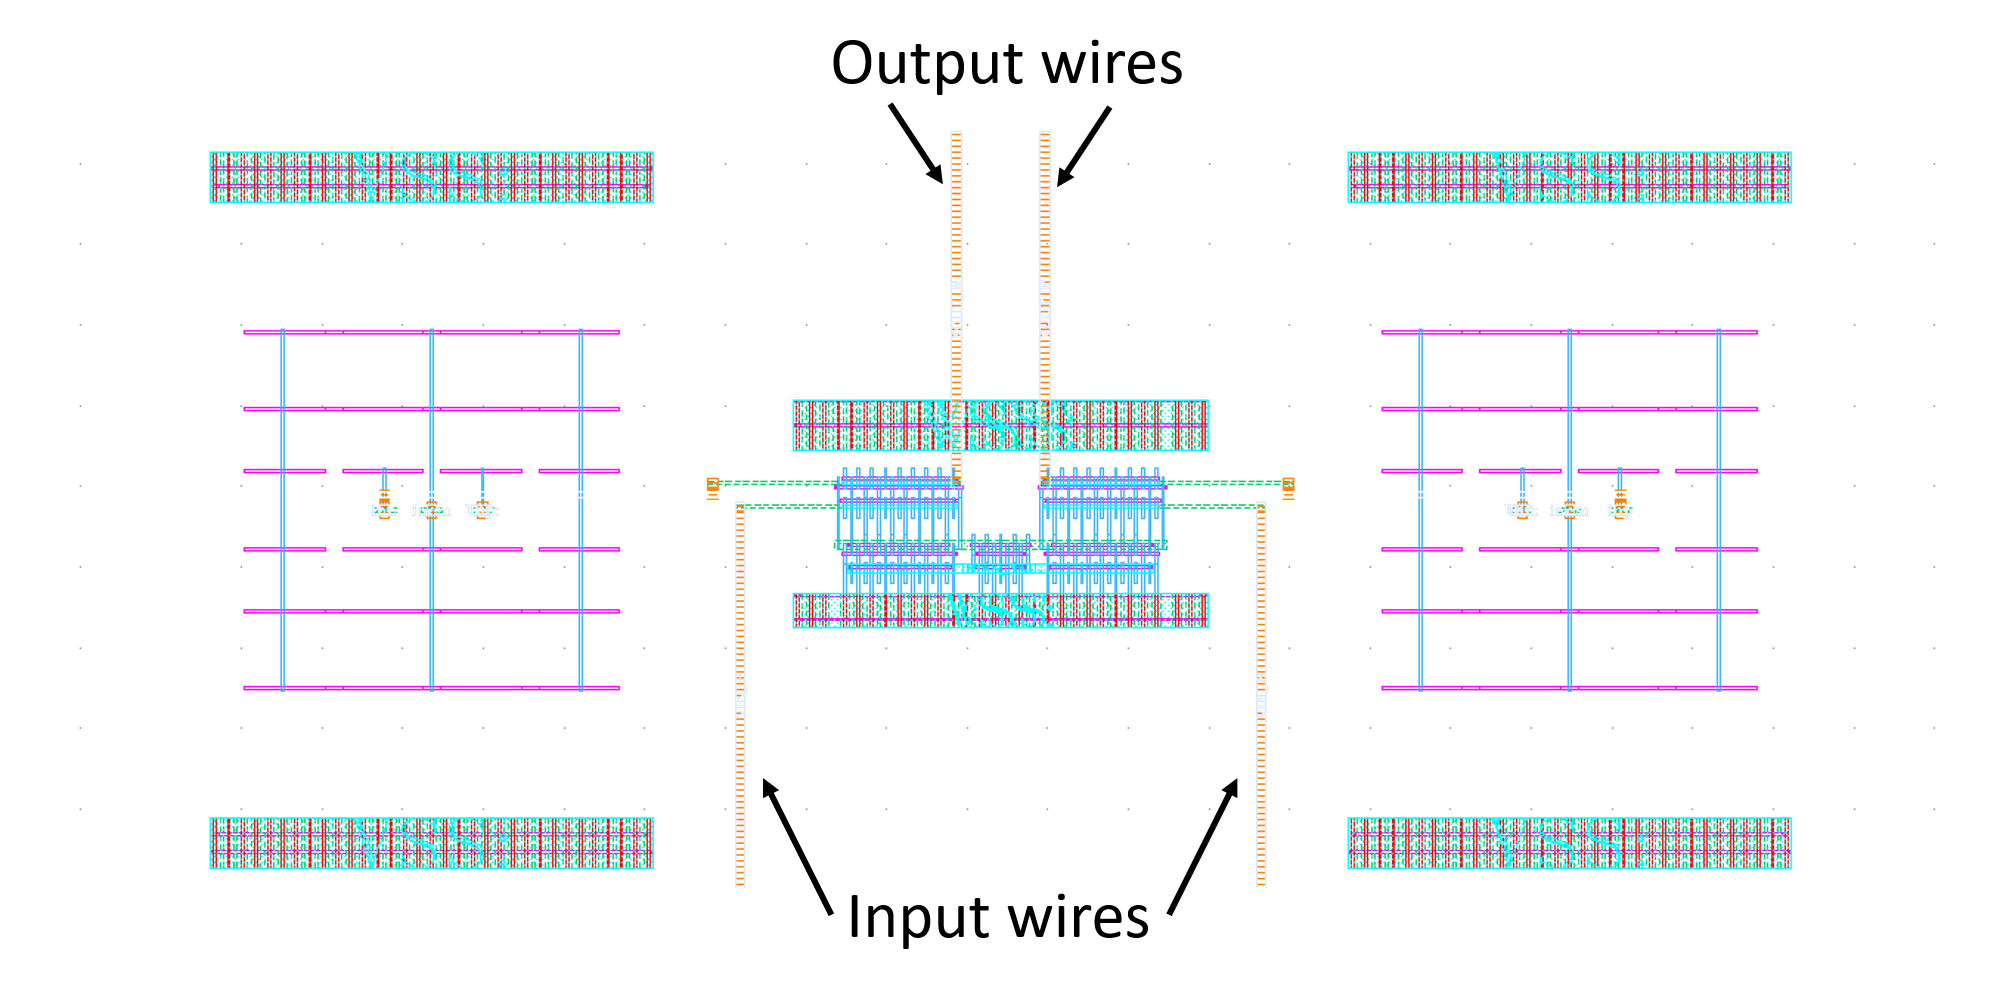
\includegraphics[width=\textwidth]{passive_layout_metals_annotated}
  \caption{Only the metals}
  \label{fig:sfig2}
\end{subfigure}
\caption{Differential amplifier layout}
\label{fig:passive_amp}
\end{figure}
All generators demonstrated have wire width parametrized so each type of wire (signal, bias, clock) can have a specific, customizable width through use of \texttt{TrackManager}. This class lets the user specify a width for each layer of interest and map them to a name. For example, if the user wants a specific width for all nets carrying a clock signal, then the user can specify the width all clock wires should be on each layer. Listing \ref{lst:tr_manager} shows a sample setup. When choosing a wire width to make a connection, the generator will select the width based on the passed specs, meaning wire widths can be parametrized as well. A section of code using this wire width is shown in \ref{lst:wire_widths}. 

This generator additionally allows the user to specify resistor unit cell sizes, number of parallel and series units and transistor dimensions (width, fingers) the same way as demonstrated in Chapter 2.
\begin{lstlisting}[language=Python, caption=Track manager setup, label={lst:tr_manager}, float]
tr_widths:
    # How wide to make the actual wires
    # format is {metal layer: track width, metal layer: width in tracks}
    bias: {4: 2, 5: 2}
    clk: {4: 1, 5: 1}
    sig: {4: 1, 5: 1}
  tr_spaces:
    # How wide to make the spaces between each wire of a certain type
    # same formatting. {metal layer: width in tracks}
    !!python/tuple ['bias', '']: {4: 1, 5: 1}
    !!python/tuple ['clk', '']: {4: 3, 5: 3}
    !!python/tuple ['clk', 'clk']: {4: 2, 5: 2}
    !!python/tuple ['clk', 'bias']: {4: 3, 5: 3}
    !!python/tuple ['sig', '']: {4: 2, 5: 2}
\end{lstlisting}
\begin{lstlisting}[language=Python, caption=Track manager usage, label={lst:wire_widths}, float]
# Create a track to put a wire on for connecting the resistor output
# terminal to the input terminal
       tid_extend_res_p_in_p = TrackID(
       #A way of specifying I want the next horizontal layer above my lowest horz. layer 
        horz_conn_layer + 2, 
        track_idx=self.grid.coord_to_nearest_track( #Helper function
            layer_id=horz_conn_layer + 2,
            #This represents the coordinate of the resistor port wire
            coord=(res_p_inp.get_bbox_array(self.grid).bottom_unit + \
                   diff_amp_vout_p.get_bbox_array(self.grid).top_unit)/2,
            unit_mode=True
        ),
        #This is where the parametrization comes in. By changing the width corresponding
        # to `bias' in the spec file, the width will automatically change here.
        width=tr_manager.get_width(horz_conn_layer+2, 'bias') 
    )
\end{lstlisting}

Another option for this generator is nearly identical, but with 3-bit resistor DACs instead of a single resistor as in Figure \ref{fig:passive_dac}
\begin{figure}[h]
\centering
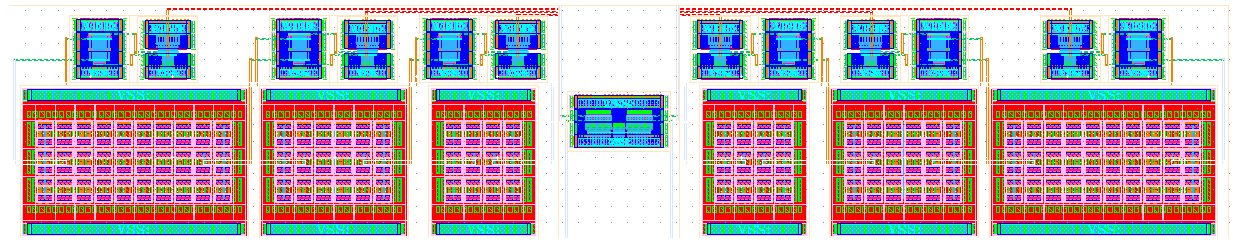
\includegraphics[width=\textwidth]{passive_dac}
\caption{Passive diff-amp with resistor DAC}
\label{fig:passive_dac}
\end{figure}

\section{Getting Fancier: A Double Tail Sense Amplifier and Latch}
Yet another crucial component in an analog receiver is the sampler. Before converting to purely digital processing, the received bits must be processed as either a 1 or a 0 through the use of a sampling circuit. While there are many ways to implement sampling, this report makes use of a double tail sense amp (DTSA) \cite{chiu_double-tail_2016}. The schematic and operation are shown in Figures 4.7 and 4.8 respectively. An example layout is shown in Figure \ref{fig:dtsa_ex}.
\begin{figure}[h]
\centering
\begin{subfigure}{.4\linewidth}
  \centering
  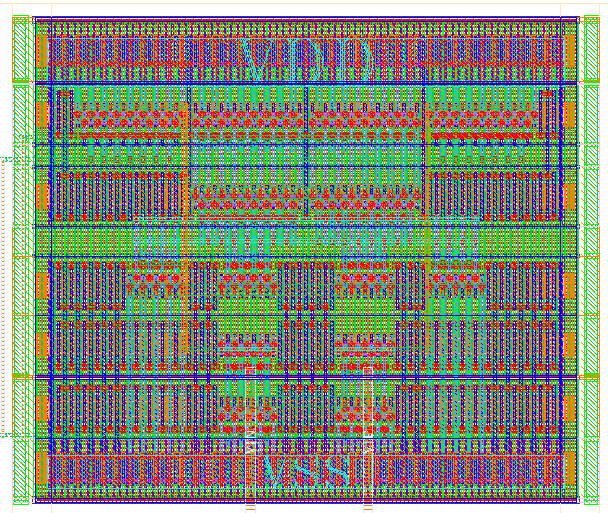
\includegraphics[width=0.8\textwidth]{dtsa_full}
  \caption{Full layout}
  \label{fig:sfig1}
\end{subfigure}
\begin{subfigure}{.4\linewidth}
  \centering
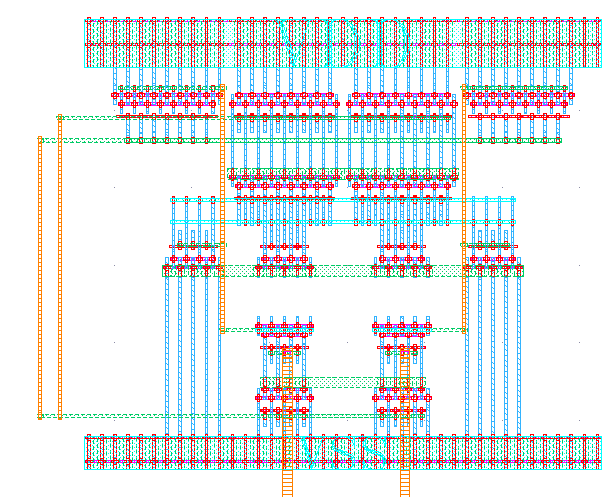
\includegraphics[width=0.8\textwidth]{dtsa_metal}
  \caption{Only the metals}
  \label{fig:sfig2}
\end{subfigure}
\caption{DTSA layout}
\label{fig:dtsa_ex}
\end{figure}
The DTSA block exemplifies even more of BAGs capability to include customization. In addition to all previously mentioned parametrization (wire widths, transistor sizings, etc.) this block also includes an option to generate input pair offset correction circuits. These circuits are implemented as a current that subtracts from the input pair's current during the integration step of operation (discussed more in  Chapter 4). The generator automatically accounts for how the setup changes when offset correction is included and automatically adds more pins/labels to the layout, as shown in Figure \ref{fig:dtsa_enoc}.
\begin{figure}[h]
\centering
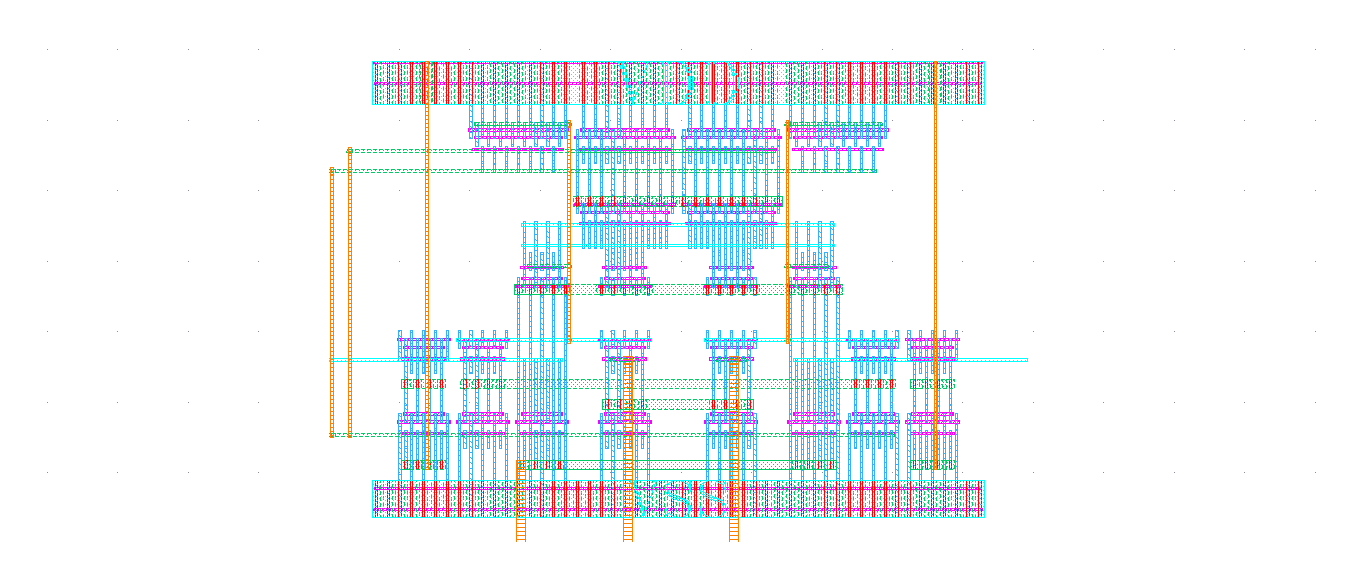
\includegraphics[width=\textwidth]{dtsa_metal_enoc}
\caption{DTSA with offset correction}
\label{fig:dtsa_enoc}
\end{figure}
Finally, the output of a comparator like this is only valid for a short time. We need a latch to store the value in between evaluation cycles. Thankfully, this is possible with BAG. Using TemplateBase we can attach a latch made previously to the output of the DTSA, like in Figure \ref{fig:dtsa_d2s}.
\begin{figure}[h]
\centering
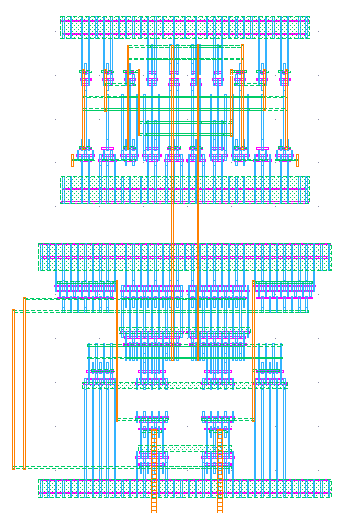
\includegraphics[width=0.4\textwidth]{dtsa_d2s}
\caption{DTSA with latch}
\label{fig:dtsa_d2s}
\end{figure}

\section{Endless Possibilities: An Entire Receiver Analog Front End Receiver or Two}
Manually creating the layout for an entire analog front-end (AFE) of the reciever is a daunting process. As a final demonstration of how a user can start with small blocks and eventually create large, complex generators, two different front end architectures are shown. It is important to note that the size and complexity of these circuits are non-trivial, and would require significant manual work. These generators are capable of creating and extracting the entire layout in seconds, which truly allows faster design iteration by removing the bottleneck almost entirely. 

The first front end (Figure \ref{fig:afe1}) is a chain of a TIA followed by a Cherry-Hooper amplifier stage, then a CTLE with resistor DACs and a capacitor DAC and two parallel preamplifiers also with resistor DAC loads. As will be discussed in Chapter 4, there are also current DACs to establish a common mode output in the first stage. 
\begin{figure}[h]
\centering
\begin{subfigure}{1\linewidth}
  \centering
  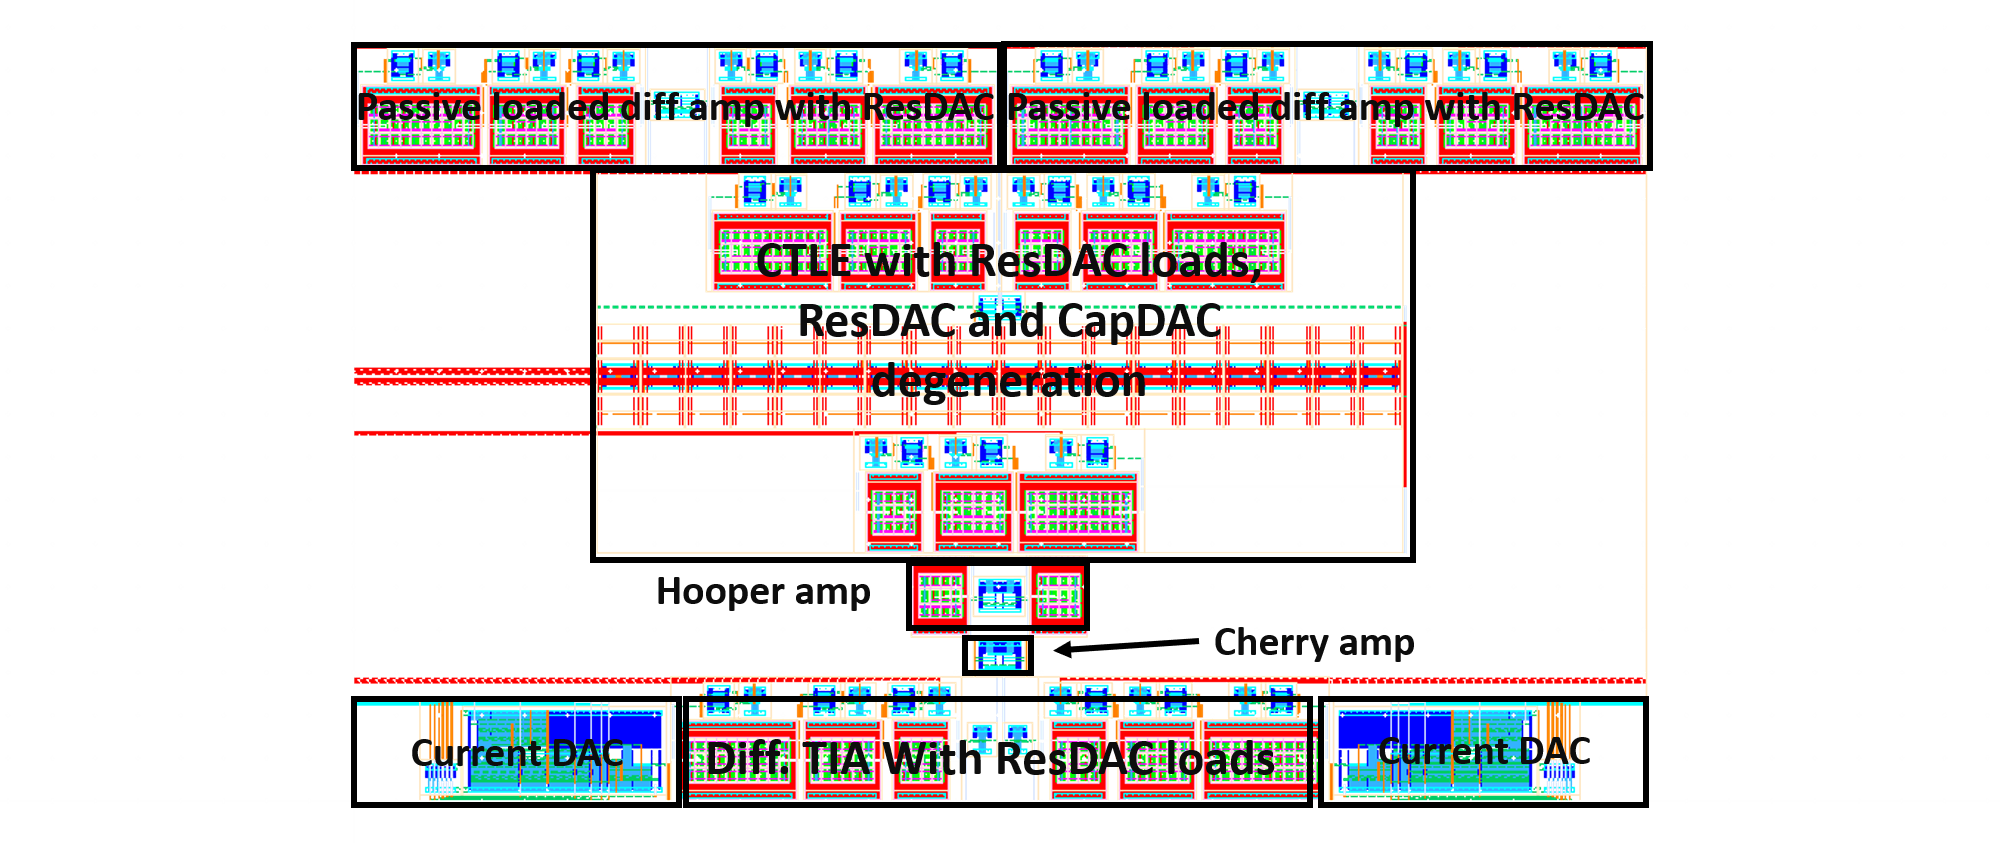
\includegraphics[width=\textwidth]{afe1_annotated}
  \caption{AFE full layout, annotated with positions of blocks}
  \label{fig:sfig1}
\end{subfigure}
\begin{subfigure}{.8\linewidth}
  \centering
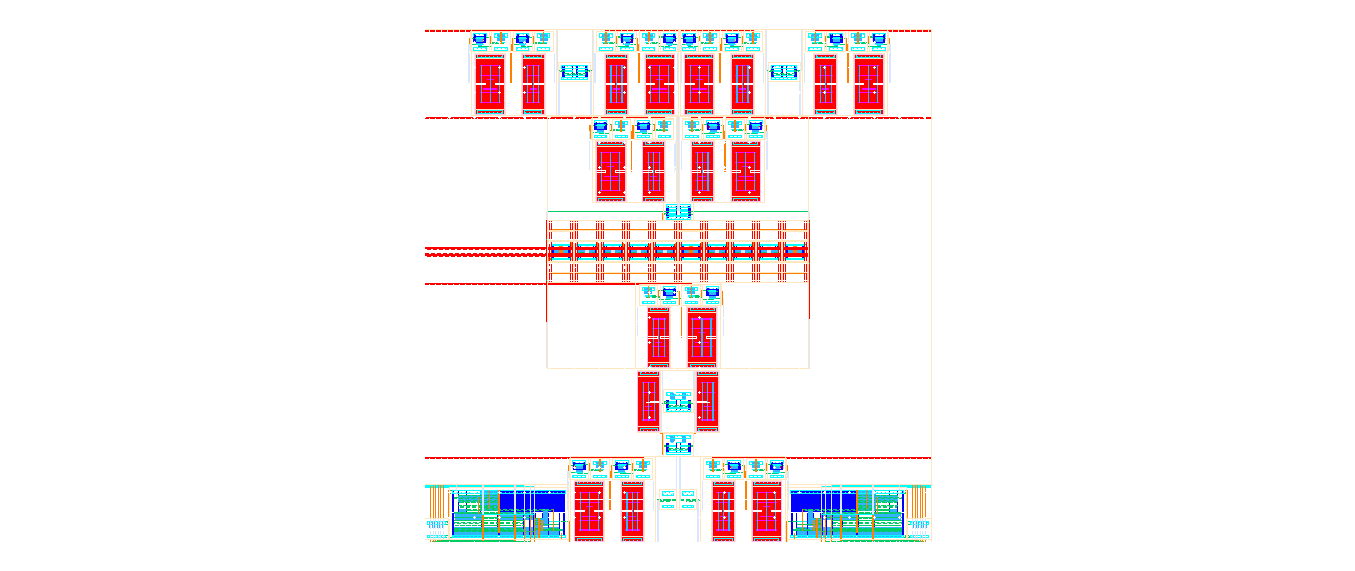
\includegraphics[width=1\textwidth]{afe1_tall}
  \caption{The same AFE with different parameters}
  \label{fig:sfig2}
\end{subfigure}
\begin{subfigure}{.8\linewidth}
  \centering
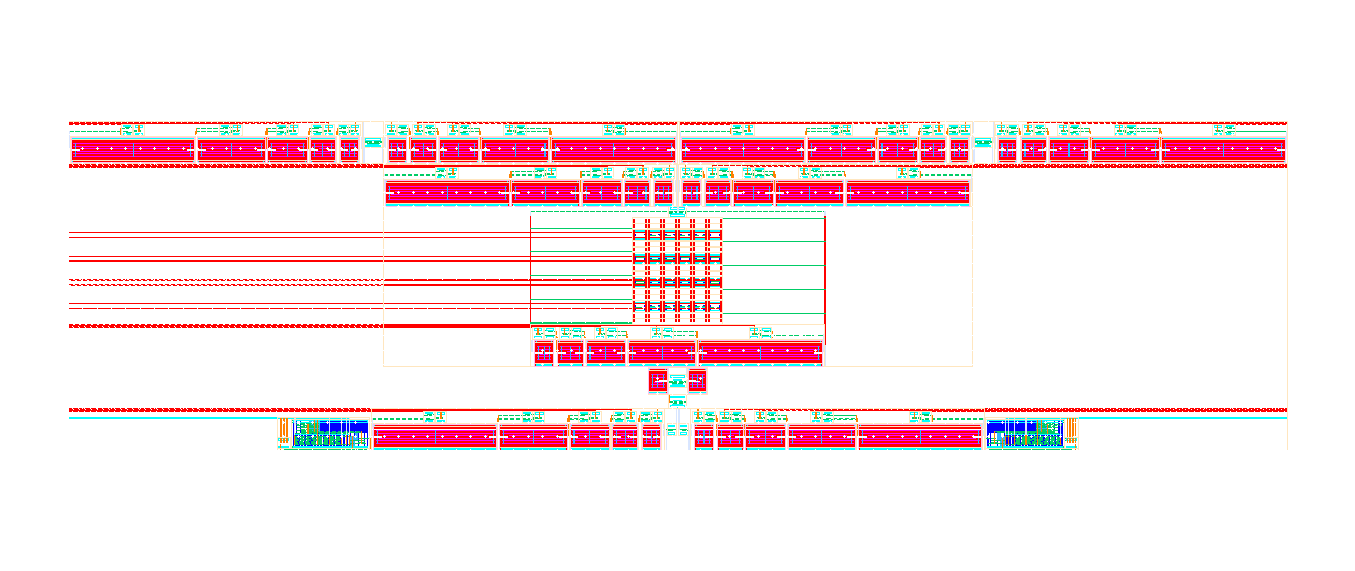
\includegraphics[width=\textwidth]{afe1_tall_wide}
  \caption{The same AFE with different parameters}
  \label{fig:sfig2}
\end{subfigure}
\caption{Various generated AFE layouts}
\label{fig:afe1}
\end{figure}
The important thing to note about these generated layouts is how much control the user has over the dimensions of the blocks. Extremely wide or tall, or balanced layouts are possible. The aspect ratio is fully customizable, and can be changed at a whim with a simple rerun of the script.

There are also versions that include DACs for every passive element as well as current DACs for every bias input. There are versions that remove the Cherry-Hooper stage and include a comparator. These various variants are also used for different simulation stages of design and verifiaction.

Another example of a front end is the one that will be used in Chapter 4. This AFE is a quad data rate AFE similar to the previous AFE and is comprised of the chain: TIA, CTLE, 2x parallel passive diff amps, 4x samplers. The architecture and operation is explained in Chapter 4. The layout is shown in Figure \ref{fig:afe2}, and of course has the same degree of customizability alluded to in this entire chapter.
\begin{figure}[h]
\centering
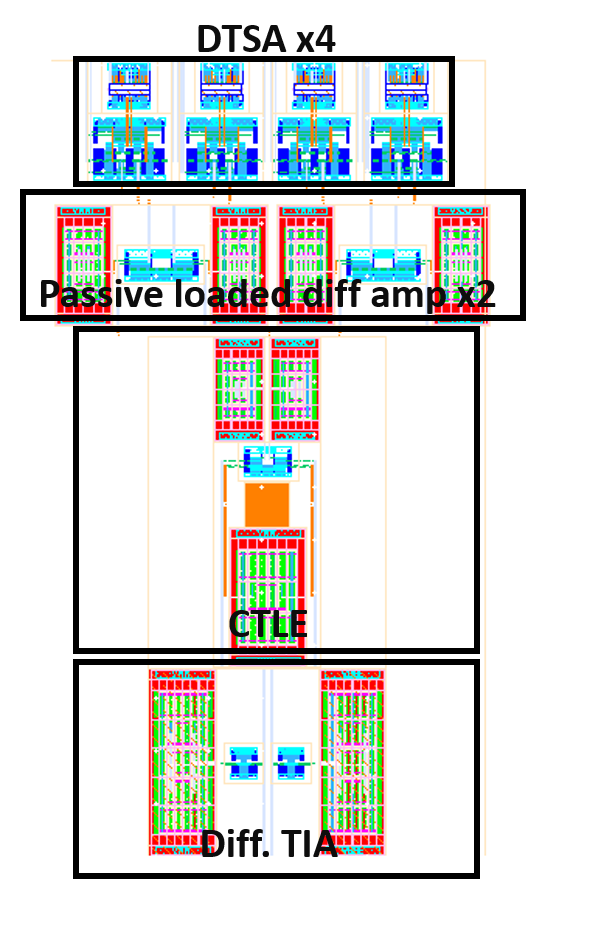
\includegraphics[width=0.5\textwidth]{afe2_annotated}
\caption{Second front end}
\label{fig:afe2}
\end{figure}
The main point of demonstrating these layouts is that with a library of ``leaf cells,'' composing large circuits is a very feasible task that would take an experienced user only one to two days to implement. With BAG, layout is no longer a painstaking process.

